\documentclass{standalone}
\usepackage{tikz}
\usepackage{ctex,siunitx}
\setCJKmainfont{Noto Serif CJK SC}
\usepackage{tkz-euclide}
\usepackage{amsmath}
\usetikzlibrary{patterns, calc}
\usetikzlibrary {decorations.pathmorphing, decorations.pathreplacing, decorations.shapes,}

\begin{document}
\small
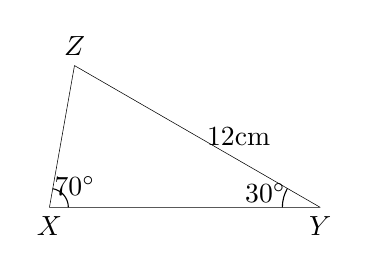
\begin{tikzpicture}[>=stealth,scale=0.6]
  \tkzSetUpPoint[fill=black]
  % \useasboundingbox(-1,-0.75)rectangle(3.7,1.4);
  \tkzDefPoints{0/0/X, 0.53/3/Z, 5.73/0/Y}
  \tkzLabelPoints[below](X,Y)
  \tkzLabelPoints[above](Z)
  \tkzLabelSegment[right](Y,Z){12cm}
  \tkzMarkAngles[size=.8, mark=none](Z,Y,X)
  \tkzMarkAngles[size=.4, mark=none](Y,X,Z)
  \tkzLabelAngle[pos=1.2](Z,Y,X){$30^{\circ}$}
  \tkzLabelAngle[pos=.7](Y,X,Z){$70^{\circ}$}
  \tkzDrawPolygon(Z,Y,X)
\end{tikzpicture}
\end{document}